%%%%%%%%%%%%%%%%%%%%%%%%%%%%%%%%%%%%%%%%%
% A beamer poster style for the University of Oxford. Atilim Gunes Baydin <gunes@robots.ox.ac.uk>, November 2016.
% Based on the I6pd2 style created by Thomas Deselaers an Philippe Dreuw.
%
% Dreuw & Deselaer's Poster
% LaTeX Template
% Version 1.0 (11/04/13)
%
% Created by:
% Philippe Dreuw and Thomas Deselaers
% http://www-i6.informatik.rwth-aachen.de/~dreuw/latexbeamerposter.php
%
% This template has been downloaded from:
% http://www.LaTeXTemplates.com
%
% License:
% CC BY-NC-SA 3.0 (http://creativecommons.org/licenses/by-nc-sa/3.0/)
%
%%%%%%%%%%%%%%%%%%%%%%%%%%%%%%%%%%%%%%%%%

%----------------------------------------------------------------------------------------
%   PACKAGES AND OTHER DOCUMENT CONFIGURATIONS
%----------------------------------------------------------------------------------------

\documentclass[final,hyperref={pdfpagelabels=false}]{beamer}

\usepackage[orientation=landscape,size=a0,scale=1.3]{beamerposter} % Use the beamerposter package for laying out the poster with a portrait orientation and an a0 paper size

\usetheme{Oxford}

\usepackage[utf8]{inputenc} % allow utf-8 input
\usepackage{blindtext}
\usepackage{amsmath,amsthm,amssymb,latexsym} % For including math equations, theorems, symbols, etc
\usepackage[document]{ragged2e}
\usepackage{times}\usefonttheme{professionalfonts}  % Uncomment to use Times as the main font
\usefonttheme[onlymath]{serif} % Uncomment to use a Serif font within math environments
%\boldmath % Use bold for everything within the math environment
\usepackage{booktabs} % Top and bottom rules for tables
\usepackage{subcaption}
\usepackage{microtype}

\usecaptiontemplate{\small\structure{\insertcaptionname~\insertcaptionnumber: }\insertcaption} % A fix for figure numbering

\newcommand{\shrink}{-15pt}

\def\imagetop#1{\vtop{\null\hbox{#1}}}

\let\oldbibliography\thebibliography
\renewcommand{\thebibliography}[1]{\oldbibliography{#1}
\setlength{\itemsep}{-10pt}}

%----------------------------------------------------------------------------------------
%   TITLE SECTION 
%----------------------------------------------------------------------------------------
\title{\Huge Variational Inference\\ with Normalizing Flows} % Poster title
%\author{Man Hon Fan, Kieran Gall, Charalampos Kokkalis, John Ryan}
%\author{1032626, 1034125, 1034129, 1036969}
\author{ATML Group 12}
\institute{Department of Computer Science, University of Oxford\\\vspace{4mm}
%\texttt{ a}
%\texttt{\{manhon.fan,kieran.gall,charalampos.kokkalis,john.ryan2\}@cs.ox.ac.uk}}
\texttt{1032626, 1034125, 1034129, 1036969}}


%----------------------------------------------------------------------------------------
%   FOOTER TEXT
%----------------------------------------------------------------------------------------
\newcommand{\leftfoot}{} % Left footer text
\newcommand{\rightfoot}{} % Right footer text


%----------------------------------------------------------------------------------------

\begin{document}
\addtobeamertemplate{block end}{}{\vspace*{2ex}} % White space under blocks

\begin{frame}[t] % The whole poster is enclosed in one beamer frame

\begin{columns}[t] % The whole poster consists of three major columns, each of which can be subdivided further with another \begin{columns} block - the [t] argument aligns each column's content to the top

  \begin{column}{.02\textwidth}\end{column} % Empty spacer column

%%%%%%%%%%%%%%%%%%%%%%%%%%%%%%%%%%%%%%%%%%
%% Column 1
%%%%%%%%%%%%%%%%%%%%%%%%%%%%%%%%%%%%%%%%%%

  \begin{column}{.3\textwidth} % 1st column

    \vspace{\shrink}          
    \begin{block}{Introduction}
      \begin{itemize}
          \item Calculating the true posterior distribution of inference tasks is in most cases an intractable problem.
          \item Lots of research on approaches for efficient approximation of the posterior, however the resulting classes prove to be of limited expressiveness.
          \item The authors in \cite{flows} introduce the notion of normalizing flows, sequences of invertible transformations applied to a simple initial density, to efficiently create more expressive families of candidate posteriors to be used for variational inference.
          \item We compare the performance of different types of normalizing flows on the MNIST dataset.
      \end{itemize}


    \end{block}

    \begin{block}{Our Work}
      \begin{itemize}
          \item Reproduced experiment on MNIST using Linear Normalizing Flows
          \item Reproduced experiment on MNIST using NICE
          \item Extended the ideas of the paper and experimented with Invertible Convolutional Flows
          \item Created open-source Github repository with code and results: \url{github.com/ATML-Group-12/normalising_flows} 
      \end{itemize}
    \end{block}

    \begin{block}{Theoretical Background}
    \textbf{Normalizing flows} are sequences of invertible, smooth mappings $f:\mathbb{R}^d\rightarrow \mathbb{R}^d$. We define a flow of length $K$ to be $K$ such transformations as follows:
    \[ \mathbf{z_K} = f_K \circ ... \circ f_2 \circ f_1 (\mathbf{z_0}) \] 
    where $\mathbf{z_0}$ is a random variable that has a simple initial distribution, and $\mathbf{z_K}$ is the corresponding random variable after applying the transformations.
    
    The properties of normalizing flows allow us to calculate the log-density of $\mathbf{z_K}$ efficiently, using the change of variable theorem:
    \[ \ln q_K(\mathbf{z_K}) = \ln q_0(\mathbf{z_0}) - \sum_{k=1}^{K} \ln \left| \det \frac{\partial f_k}{\partial \mathbf{z_{k-1}}} \right| \]
    The normalizing flow is defined as the path of the successive distributions $q_K$.
    
    The first class of flows that we use in our experiments is that of linear flows. More specifically, we consider \textbf{planar} and \textbf{radial} flows, which perform series of contractions and expansions in the direction perpendicular to a fixed hyperplane and around a reference point respectively.
          
    \end{block}
  \end{column} % End of the 1st column

%%%%%%%%%%%%%%%%%%%%%%%%%%%%%%%%%%%%%%%%%%
%% Column 2
%%%%%%%%%%%%%%%%%%%%%%%%%%%%%%%%%%%%%%%%%%

  \begin{column}{.02\textwidth}\end{column} % Empty spacer column

  \begin{column}{.3\textwidth} % 2nd column
    \vspace{\shrink}
    \begin{block}{Theoretical Background}
      The authors compare their work with \textbf{NICE}, which introduces coupling layers. A coupling layer $f$ is a neural network layer with easy to compute inverse and a trivial Jacobian. For an input vector $\mathbf{z} \in \mathbb{R}^D$, we have
\begin{equation}
f(\mathbf{z}) = (\mathbf{z}_A, g(\mathbf{z}_B,h(\mathbf{z}_A))) 
\end{equation}
\begin{equation}
f^{-1}(\mathbf{z}) = (\mathbf{z}_A, g^{-1}(\mathbf{z}_B,h(\mathbf{z}_A)))
\end{equation}
where $(A,B)$ is a partition of $\{1,2,\dots,D\}$, $h$ is a neural network with input size $|A|$, and $g$ is a coupling law, a function that is invertible for the first argument given the second. When $g(a,b)=a+b$, the Jacobian is the identity matrix, so $f$ is classified as a volume-preserving flow.
\end{block}

    
          
      \begin{block}{Experiments}
     	We compare expressivity of normalizing flows with NICE coupling layers. We also added in diagonal scaling for NICE layers since this was not accounted for in the original results.
      \end{block}
      
      \begin{center}
	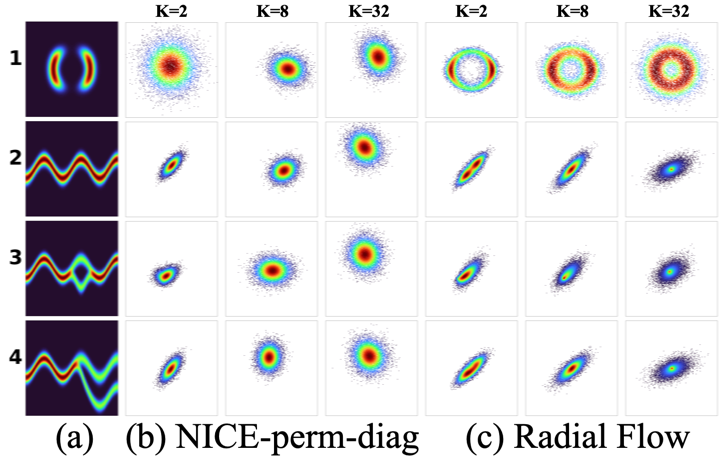
\includegraphics[width=0.9\columnwidth]{EFs-ours}
      \end{center}
      
      	\begin{center}
        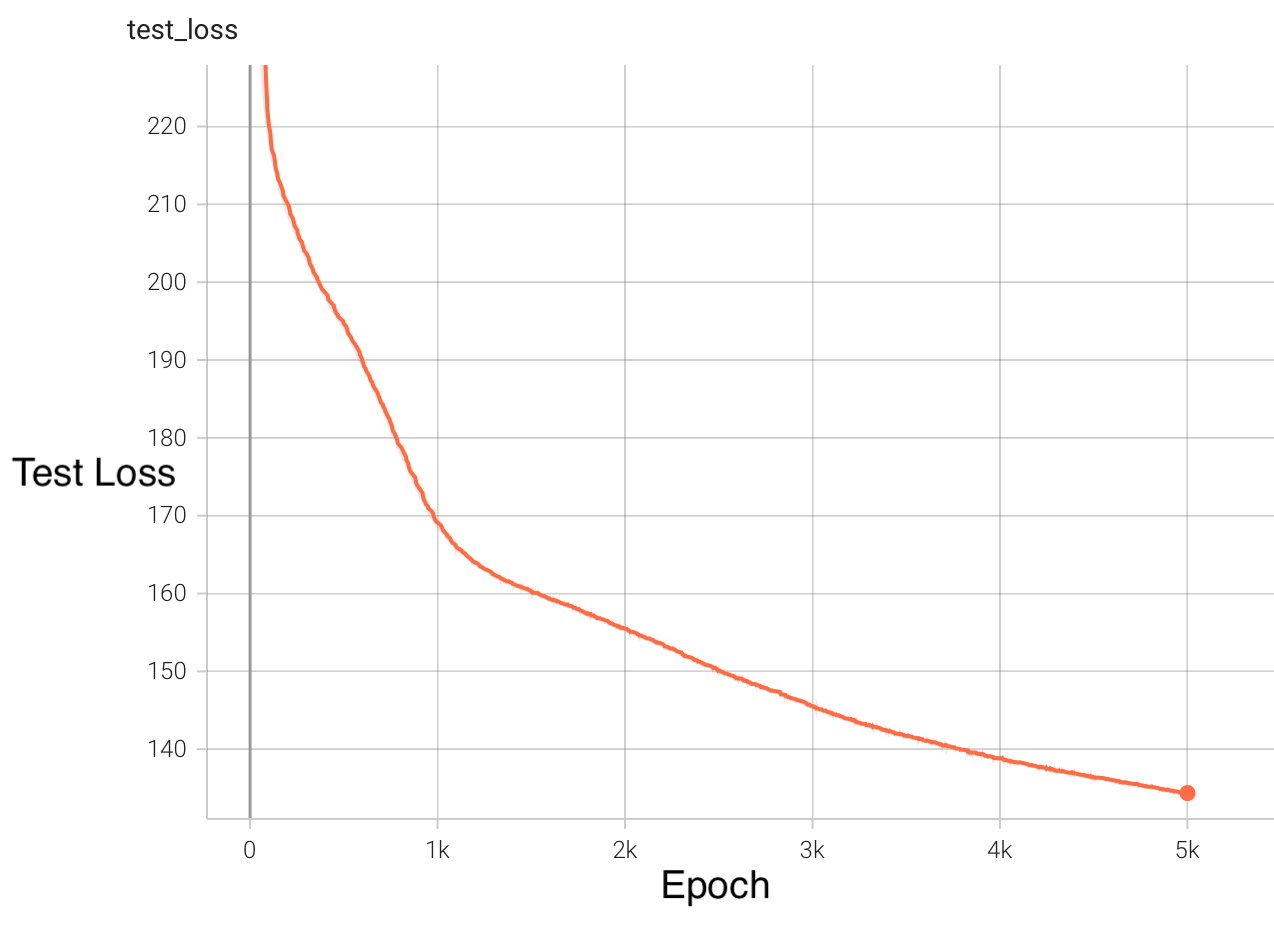
\includegraphics[width=0.5\columnwidth]{circular_conv_test_loss.png}\\
        \textit{Figure: Test Loss over 5000 epochs using Circular Convolutional Flows}
      \end{center}
      
      
    

  \end{column} % End of the 2nd column
  

%%%%%%%%%%%%%%%%%%%%%%%%%%%%%%%%%%%%%%%%%%
%% Column 3
%%%%%%%%%%%%%%%%%%%%%%%%%%%%%%%%%%%%%%%%%%

  \begin{column}{.02\textwidth}\end{column} % Empty spacer column

  \begin{column}{.3\textwidth} % 3rd column

    \vspace{\shrink} 
   \begin{block}{Results}
      The range of variational bounds is close to those from the paper, but the shapes are visibly inconsistent. We suspect this is due to the ``parameter updates" being iterations or epochs, as well as the model being not well-specified in the paper. We do note that among NICE-based models, those with diagonal scaling do perform better than their counterparts.
      \end{block}
    
      \begin{figure}
     	\centering
	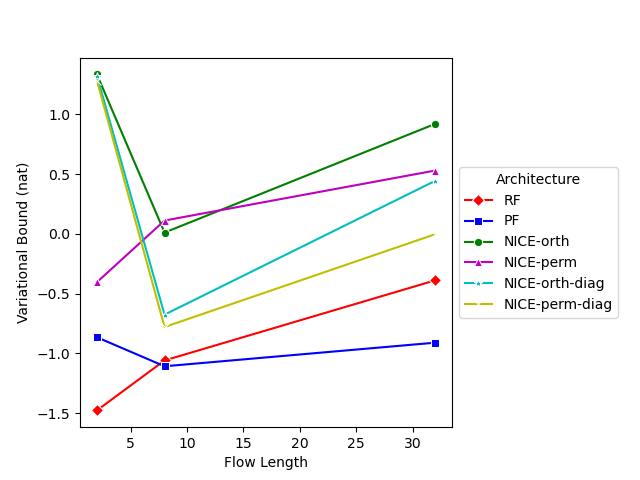
\includegraphics[width=0.45\columnwidth]{u1}
	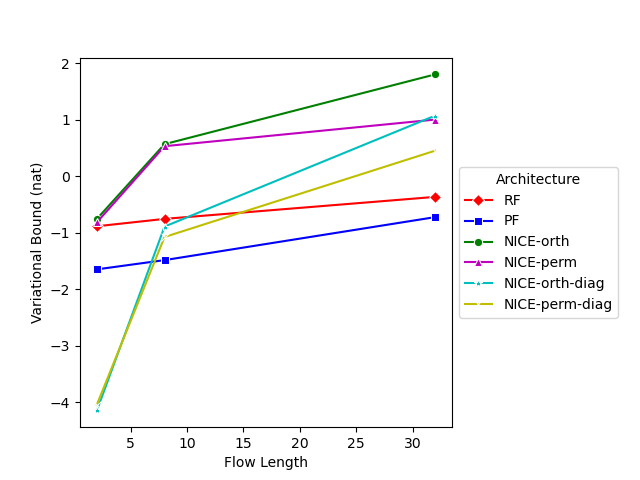
\includegraphics[width=0.45\columnwidth]{u2}
	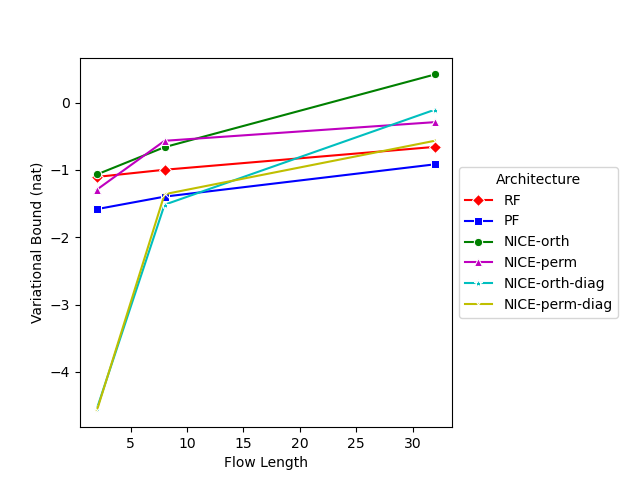
\includegraphics[width=0.45\columnwidth]{u3}
	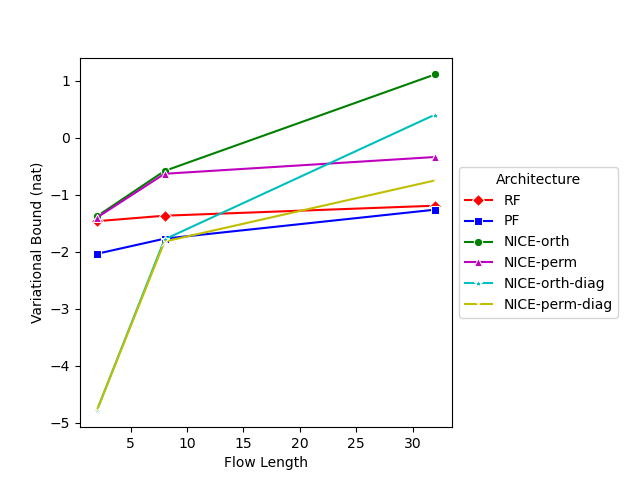
\includegraphics[width=0.45\columnwidth]{u4}
	\caption{(d) Variational bounds}
      \end{figure}
    
    
    \begin{block}{Our Improvements and Extensions}
    
	To extend the results of the paper, we also looked to what other kinds of flows we could implement.
	The authors of Invertible Convolutional Flows have used transformations whose determinants are \textit{circulant matrices}, which will allow computation of the log determinant, as well as the convolution and its inverse, to be calculated in time $\mathcal{O}(N \log N)$ by making use of Discrete Fourier Transforms (DTFs). Since it had no public implementations, we decided to implement this - Circular Convolutional Flows.
	
	
	\end{block}
	


    \begin{block}{References}
      \nocite{*} % Insert publications even if they are not cited in the poster
      \linespread{0.928}\selectfont
      \footnotesize{\bibliographystyle{unsrt}
      \bibliography{poster}}
    \end{block}

  \end{column} % End of the 3rd column

  \begin{column}{.02\textwidth}\end{column} % Empty spacer column

\end{columns} % End of all the columns in the poster

\end{frame} % End of the enclosing frame

\end{document}
